\documentclass{beamer}
\usetheme{UWr_white}

\usepackage [utf8]{inputenc}
\usepackage {color,graphicx}
\usepackage {amssymb}
\usepackage {enumerate}
\usepackage {amsmath}
\usepackage {caption}
\usepackage {subcaption}
\usepackage {geometry}
\usepackage {empheq}
\usepackage {wrapfig}
\usepackage {float}

\title{Przykładowa prezentacja tematu WFA}
\author{Krzysztof Cach}
\institute{Instytut fizyki teoretycznej}
\date{Wrocław, \today}

\setbeamercovered {invisible}

\begin{document}

\begin{frame}
	\titlepage{}
\end{frame}

\begin{frame}
\frametitle{Przykładowe elementy:}
\tableofcontents
\end{frame}

\section{Enumerate}
\begin{frame}
	\frametitle{Enumerate}
	\begin{enumerate}
	\item item1
		\begin{enumerate}
		\item item1a
			\begin{enumerate}
				\item item1
				\item item2
					\item item3
			\end{enumerate}

		\item item2a
		\item item3a
	\end{enumerate}
	\item item2
	\item item3
	\end{enumerate}
\end{frame}

\section{Itemize}
\begin{frame}
	\frametitle{Itemize}
	\begin{itemize}
	\item item1
		\begin{itemize}
			\item item1a
			\begin{itemize}
				\item item1
				\item item2
				\item item3
			\end{itemize}
			\item item2b
			\item item3c
		\end{itemize}
	\item item2
	\item item3
	\end{itemize}
\end{frame}

\section{Blocks}
\subsection{alert}
\subsection{standard}
\subsection{example}

\begin{frame}
	\frametitle{Blocks}
	\begin{alertblock}{Alert block}
		Body
	\end{alertblock}

	\begin{block}{Standard block}
		Body
	\end{block}

	\begin{exampleblock}{Example block}
		Body
	\end{exampleblock}
\end{frame}

\begin{frame}
Beamer is a LaTeX class for creating slides for presentations. It supports both pdfLaTeX and LaTeX + dvips. The name is taken from the German word Beamer, a pseudo-anglicism for video projector.

The beamer class is not the first LaTeX class for creating presentations, and like many of its predecessors, it has special syntax for defining 'slides' (known in Beamer as 'frames'). Slides can be built up on-screen in stages as if by revealing text that was previously hidden or covered. This is handled with PDF output by creating successive pages that preserve the layout but add new elements, so that advancing to the next page in the PDF file appears to add something to the displayed page, when in fact it has redrawn the page.

Source code for beamer presentations, like any other LaTeX file, can be created using any text editor, but there is specific support for beamer syntax in AUCTEX and LyX.
\end{frame}

\section{Equation}
\begin{frame}
	\frametitle{Equation}
	\begin{equation}
	\theta_i(t + \delta t) = \left< \theta (t) \right> _{S(i)} + \xi
	\end{equation}
	
	\begin{equation}
	\Phi = \frac{1}{N} \left| \sum_j \vec{v}_j \right|
	\end{equation}
\end{frame}

\section{Graphics}
\begin{frame}
	\frametitle{Graphics}
	\begin{figure}[H]
	\caption{Czirók, Vicsek - Physica A 281 (2000) 17-29}
	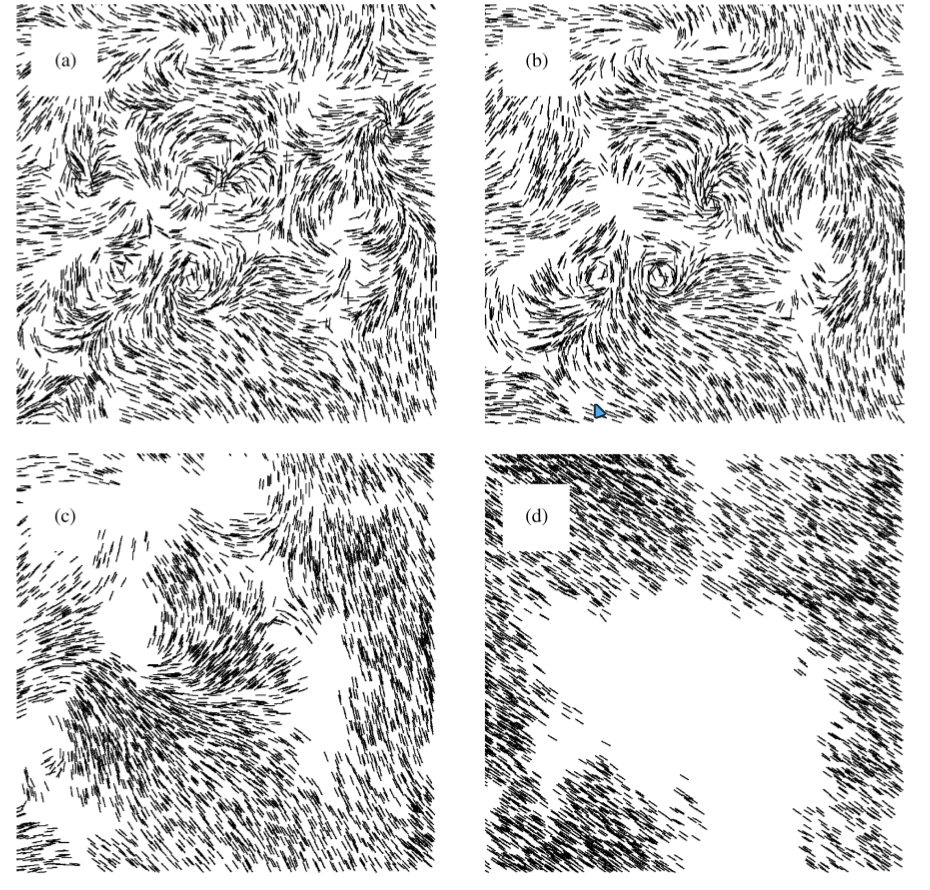
\includegraphics[width=0.7\textwidth, height=0.7\textheight]{images/wyniki.png}
	\end{figure}	
\end{frame}
\end{document}
